\section{Custom Image Compression (jc)}
\label{Custom_comp_research}

Before starting research into image compression standards such as jpeg, a range of general image compression techniques were researched and a selection of these were also implemented in MATLAB, see appendix \ref{chap:Matlab_code}.

\subsection{Overview of Available Methods (jc)}

The idea of image compression is to reduce the amount of data used to describe the image, whilst retaining as much as possible of the information contained in the image. there are two main types of image compression: lossless and lossy.

Lossless compression techniques retain all the information in the image but reduce the size of the data required to describe it, although they can't achieve the same level of compression as lossy techniques. This is usually done by looking for patterns in the data and using these patterns to encode the data in a more efficient way. Some examples of lossless techniques are: run-length encoding or entropy encoding (such as huffman encoding, see section \ref{sec:mikes_huff}). \cite{image_compression}

Lossy compression techniques discard some of the information in the image in order to be able to compress it further than is possible with lossless compression. The two main types of lossy image compression are those based on reducing the information in the colour space (often utilising the way the human eyes works in order to maintain perceived image quality) and those based on transforming the image, usually into a version of the frequency space. \cite{image_compression}

If the image is being compressed so that it can be sent over a medium then this can be done either as a single action: the image is compressed and sent once and any information that is lost is lost forever, or progressively: the image is compressed first with a high loss of information and then the additional information is sent so that the loss of the image being sent reduces as more data is received.

Reducing the resolution of an image could also be considered as lossy compression as it is a very simple method of reducing the amount of data required to describe an image by reducing the information in the image.

\subsection{Downsampling (jc)}
\label{downsampling}

The most obvious method for sending an image progressively is to simply send pixels in such an order that at any time they form a down sampled (lower resolution) version of the image. This way rather than having the image fill in from the top left hand corner the image can become less pixelated as more data is downloaded.

%[] diagram showing how this could work []

%Figure [] ref to above [] show one method that could be used to reconstruct the image progressively.

\subsection{Mike's huffman shizz (mike)} %working title :P
\label{sec:mikes_huff}

\subsection{Mitch's colour space and croma subsampling shizz (mitch)} %also a working title
\label{sec:mitch_colour}

\subsection{Transform Based Compression (jc)}
\label{transfom_based}

Some simple progressive encoding was done as an investigation into using the fast fourier transform (FFT) and the discrete cosine transform (DCT) for image compression and how these could be sent progressively.

The fourier transform works by approximating a signal with the sum of sinusoids of different frequencies. The transform function (given an array as an input) outputs an array of complex numbers whose magnitude is the magnitude of the sinusoid at that frequency and whose argument is the phase.

The fast fourier transform (FFT) is an optimised version of the discrete fourier transform (DFT) which implements the fourier transform in discrete rather than continuous space, this enables its implementation by computers.

\begin{equation}
X(k) = \sum_{j=1}^N x(j)\omega _N ^{(j-1)(k-1)}
\label{FFT1_eq}
\end{equation}

where
$ \omega _N = e^{(-2 \pi i)/N} $ is an $N$th root of unity.

Equation \ref{FFT1_eq} is the equation for the 1 dimensional FFT, to implement the FFT in 2 dimensions (as you would need to for an image) you simply take the 1 dimensional FFT of each column and then of each row of the result.

The DCT approximates a signal with the sum of cosine functions of different frequencies. The DCT is similar to the FFT in that it transforms into a frequency space, but the DCT produces strictly real values.

\begin{equation}
F_{u,v} = \alpha(x) \alpha(y) \sum_{x=0}^{M-1} \sum_{y=0}^{N-1} f_{x,y} \cos\Big[\dfrac{\pi}{M}(u+\dfrac{1}{2})x\Big]\cos\Big[\dfrac{\pi}{N}(v+\dfrac{1}{2})y\Big]
\label{DCT2_eq}
\end{equation}

for $0 \leq u \leq M - 1 $ and $0 \leq v \leq N - 1 $

$x$ is the pixel row

$y$ is the pixel column

$u$ is the horizontal DCT frequency

$v$ is the vertical DCT frequency

$
  \alpha(x) = \left\{
  \begin{array}{l l}
    1/ \sqrt{M} & \quad \text{, $u = 0$}\\
    2/ \sqrt{M} & \quad \text{, $1 \leq u \leq M - 1$}\\
  \end{array} \right.
$

$
  \alpha(y) = \left\{
  \begin{array}{l l}
    1/ \sqrt{N} & \quad \text{,$ v = 0$}\\
    2/ \sqrt{N} & \quad \text{, $1 \leq v \leq N - 1$}\\
  \end{array} \right.
$

The 2 dimensional DCT equation is given in equation \ref{DCT2_eq}, this is the equation exactly as implemented in the MATLAB function "dct2" used in [] ref to matlab code in appendix [].

\subsubsection{Whole Image (jc)}

The first algorithm to be implemented was a progressive scheme based on taking an FFT of the whole image and then reconstructing the image using more and more of the frequency content of the image starting with the lowest frequencies.

\begin{figure}[H]
  \centering
  \begin{tabular}{c c c}
  \subfigure[Image with only low frequency content]{\label{fig:whole_fft_lfc}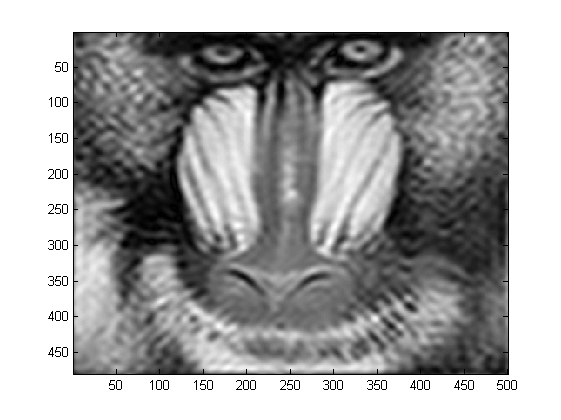
\includegraphics[width=0.3\textwidth]{figures/whole_fft_lfc.png}}&                
  \subfigure[Image with medium and low frequency content]{\label{fig:whole_fft_mfc}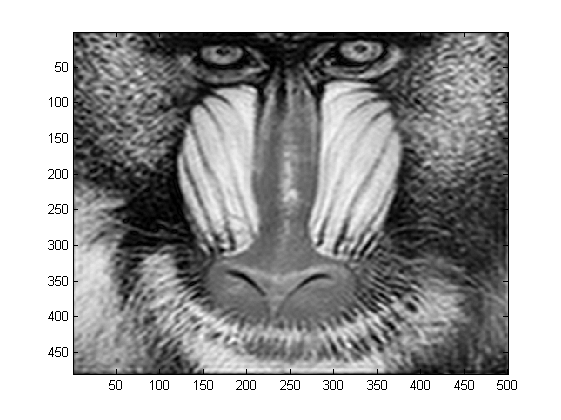
\includegraphics[width=0.3\textwidth]{figures/whole_fft_mfc.png}}&
  \subfigure[Image with all its frequency content]{\label{fig:whole_fft_all}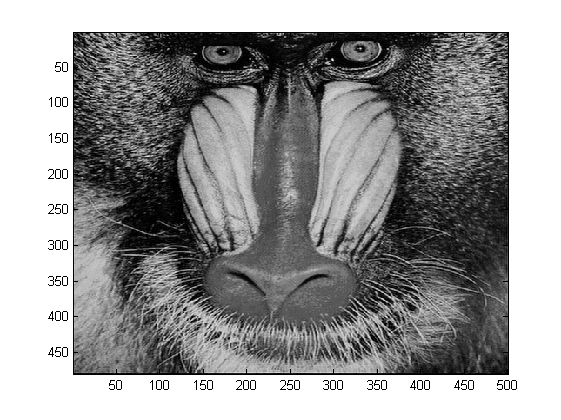
\includegraphics[width=0.3\textwidth]{figures/whole_fft_all.png}}
  \end{tabular}
  \captionof{figure}{Images reconstructed from increasing amounts of an fft of the whole image, generated by [] ref to matlab code []}
  \label{fig:whole_fft}
\end{figure}

Figure \ref{fig:whole_fft} how the level of detail in the picture increases as more of the frequency content is used to display it. Potentially the image data could be transmitted so that the low frequency data is received first and additional frequency content is then sent progressively so that the image gains detail smoothly.

The algorithm was then implemented again but using the the DCT rather than the FFT. The advantage of the DCT over the FFT for this purpose is that the FFT generates complex values thereby effectively doubling the amount of data whereas the the DCT only produces real values.

\begin{figure}[H]
  \centering
  \begin{tabular}{c c c}
  \subfigure[Image with only low frequency content]{\label{fig:whole_dct_lfc}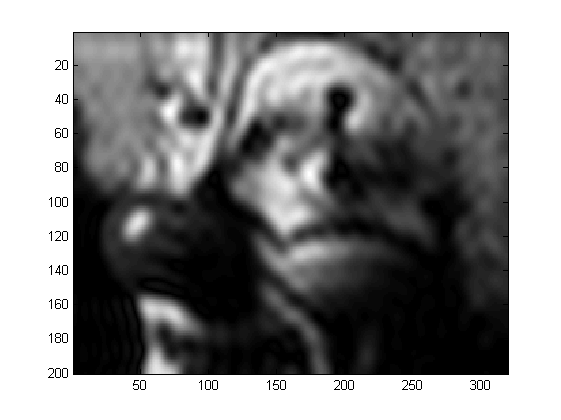
\includegraphics[width=0.3\textwidth]{figures/whole_dct_lfc.png}}&                
  \subfigure[Image with medium and low frequency content]{\label{fig:whole_dct_mfc}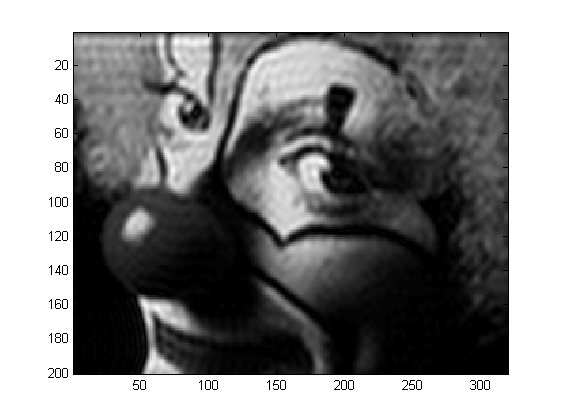
\includegraphics[width=0.3\textwidth]{figures/whole_dct_mfc.png}}&
  \subfigure[Image with all its frequency content]{\label{fig:whole_dct_all}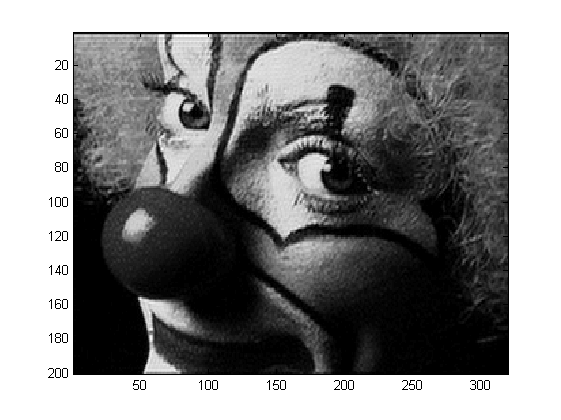
\includegraphics[width=0.3\textwidth]{figures/whole_dct_all.png}}
  \end{tabular}
  \captionof{figure}{Images reconstructed from increasing amounts of a dct of the whole image, generated by [] ref to matlab code []}
  \label{fig:whole_dct}
\end{figure}

\subsubsection{Sectioned Image (jc)}

As FFTs or DCTs can be quite computationally intensive when done with large arrays of values it was decided that it would be sensible to first break the image down into smaller blocks and then do the transformation on these. This would reduce the complexity of the computations while retaining the same functionality.

\begin{figure}[H]
  \centering
  \begin{tabular}{c c c}
  \subfigure[Sectioned image with only low frequency content]{\label{fig:sectioned_fft_lfc}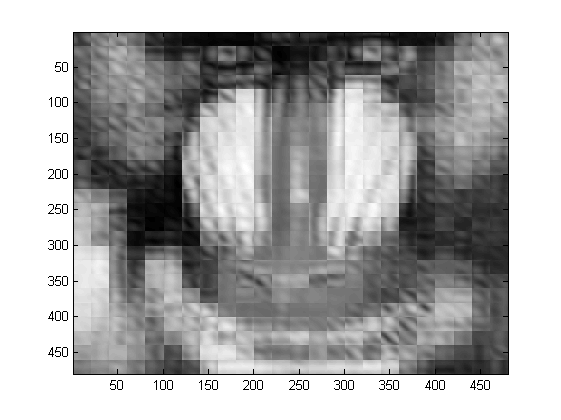
\includegraphics[width=0.3\textwidth]{figures/sectioned_fft_lfc.png}}&                
  \subfigure[Sectioned image with medium and low frequency content]{\label{fig:sectioned_fft_mfc}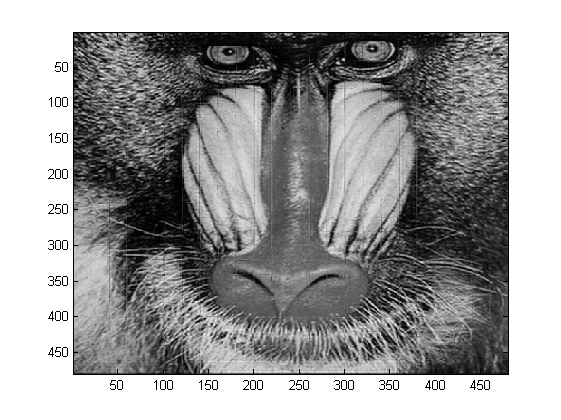
\includegraphics[width=0.3\textwidth]{figures/sectioned_fft_mfc.png}}&
  \subfigure[Sectioned image with all its frequency content]{\label{fig:sectioned_fft_all}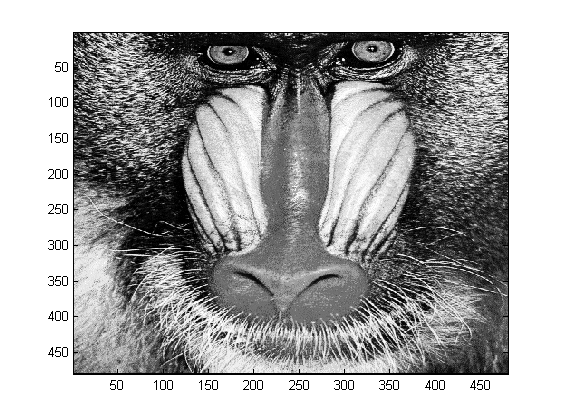
\includegraphics[width=0.3\textwidth]{figures/sectioned_fft_all.png}}
  \end{tabular}
  \captionof{figure}{Images reconstructed from increasing amounts of a fft of sections of the image, generated by [] ref to other matlab code []}
  \label{fig:sectioned_fft}
\end{figure}

Figure \ref{fig:sectioned_fft} shows much the same as figure \ref{fig:whole_fft} but with the image first broken down into small (definable in the code (see [] ref to matlab code []), 20x20 blocks were used for these images) sections and then the frequency components of these transmitted progressively so that the detail within each section increases as more data is sent and thus the detail of the whole image also increases.